%% Source: https://github.com/tias/constraint-solving-course
%% Licensed under CC BY-NC-SA 4.0: https://creativecommons.org/licenses/by-nc-sa/4.0/
%% You may share and adapt this for non-commercial use,
%% with attribution and under the same license.

\documentclass{cons-beamer}

\begin{document}


\begin{frame}{L06: Symmetry and dominance breaking}
  \begin{center}
    ~ \\
    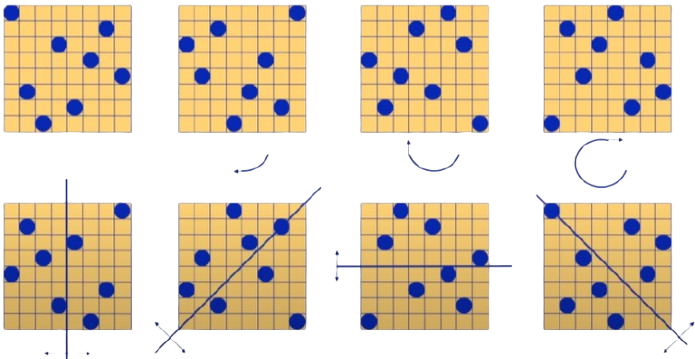
\includegraphics[height=34mm]{images/nqueens3.png} \\
    \vfill
    Prof. Tias Guns and Dr. Dimos Tsouros \\[0.5em]
    
\includegraphics[width=2cm]{images/kuleuven_CMYK_logo.pdf}
  \end{center}
  
  {\footnotesize 
  Partly based on slides from Pierre Flener, Uppsala University.}
  % https://pierre-flener.github.io/courses/M4CO/lectures.html
\end{frame}


\section{Introduction}

\begin{frame}{Quick Recap}
  \begin{enumerate}
    \item \inference{Modelling}: express problem in terms of \vfill
      \begin{itemize}
      \item parameters, \vfill
      \item decision variables, with their domains \vfill
      \item constraints, and \vfill
      \item (optionally) objective.
      \end{itemize} \vfill
    \item \search{Solving}: solve using a state-of-the-art solver.
  \end{enumerate}
\end{frame}

\begin{frame}{From a Problem to a Model} 
  What is a good model for a constraint problem? \vfill
  \begin{itemize}
    \item A model that \alert{correctly} represents the problem. \vfill
    \item A model that is \alert{easy} to understand and maintain. \vfill
    \item A model that is solved \alert{efficiently}. \vfill
  \end{itemize}\vfill
\end{frame}

\begin{frame}{Modelling}
  Modelling is still more a craft than a science: \vfill
  \begin{itemize}
    \item Choice of \textbf{viewpoint}: which are the decision variables and their domains? 
      \begin{itemize}
        \item Use of \textbf{auxiliary} variables \dots
        \item \textbf{Channel} different viewpoints \dots
      \end{itemize} \vfill
    \item Choice of the constraint formulations 
      \begin{itemize}
        \item Use \textbf{implied} constraints to reduce the search space \dots
      \end{itemize} \vfill
    \item Choice of solver and solver configuration 
  \end{itemize}
  \vfill

  \alert{Make a model correct before making it efficient!}
\end{frame}

\begin{frame}{Making an efficient model} 
  Implied constraints can reduce the search space.

  \begin{definition}[recap]
      \defined{Implied constraints}, also called \textit{redundant} constraints, are constraints that are entailed by the constraints defining the problem. They do \textbf{\textit{not change the set of solutions}}, and hence are logically redundant.
  \end{definition}
  \vfill 

  Is there any other way to \red{reduce the search space}, making the model more efficient?
\end{frame}

\begin{frame}{Example: graph colouring}
  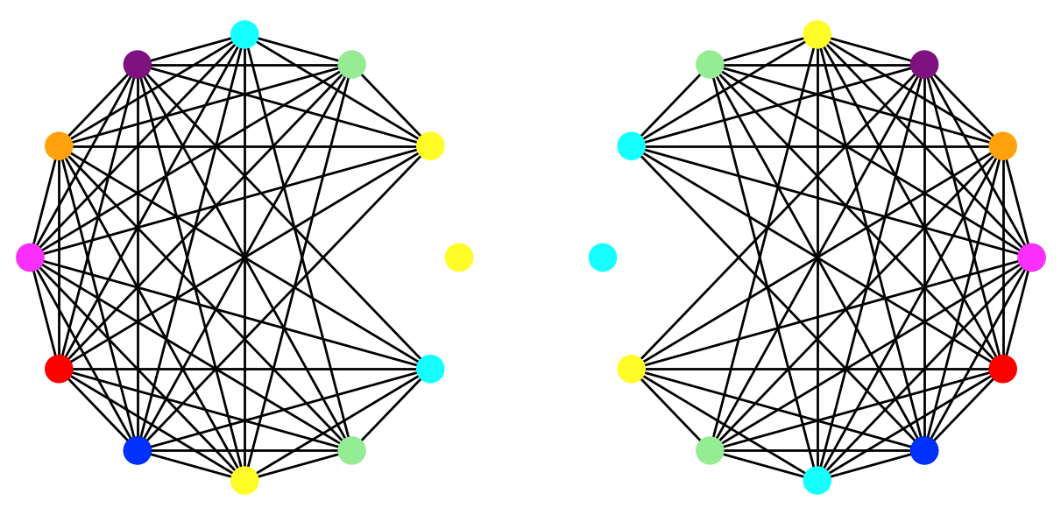
\includegraphics[height=58mm]{images/graph_pm_symmetric} 
  \vfill 

  \structured{Exploit the problem symmetries!}
\end{frame}


\section{Symmetries}

\begin{frame}{Symmetries}
  Symmetries are defined    
  based on the concept of \defined{permutation}; permuting elements of a group of variables or values can lead to symmetric solutions!
  \vfill

  \begin{definition}
    A \defined{permutation} $\pi$ over a discrete \textit{set} $D$ is a 1-1 function from $D$ to $D$. It is an arrangement of the elements of the set in a specific order.
  \end{definition}
  \vfill

  \begin{itemize}
    \item[\textcolor{red}{$\blacksquare$}] Intuitively: just a re-arrangement of the elements. E.g.:
  \end{itemize}

  \[
  \begin{aligned}
      i &: \ (1 \quad 2 \quad 3 \quad 4 \quad 5) \\
      \pi(i) &: \ (4 \quad 3 \quad 2 \quad 1 \quad 5)
  \end{aligned}
  \]
\end{frame}

\begin{frame}{Symmetries}
  \begin{definition}%[also see Cohen et al. @ \emph{Constraints}, 2006]
    A \defined{symmetry} $\sigma$ is a permutation of values or decision
    variables (or both) \\ that \defined{preserves all constraints and solutions}: it
    transforms (partial) solutions into (partial) solutions, and it
    transforms (partial) non-solutions into (partial) non-solutions.
  \end{definition}
  \vfill

  \begin{example}
    \footnotesize
    Assume a problem with 5 variables, that has 1 variable symmetry $\sigma$:
    \[
    \begin{aligned}
      i &: \ (x_1 \quad x_2 \quad x_3 \quad x_4 \quad x_5) \\
      \sigma(i) &: \ (x_4 \quad x_3 \quad x_2 \quad x_1 \quad x_5)
    \end{aligned}
    \]
    Based on the symmetry $\sigma$, each solution: 
    $(x_1=v_1 \quad x_2=v_2 \quad x_3=v_3 \quad x_4=v_4 \quad x_5=v_5)$
    \\[+5pt]
    can be transformed to a symmetric solution: \\
    $(\sigma(x_1)=v_1 \quad \sigma(x_2)=v_2 \quad \sigma(x_3)=v_3 \quad \sigma(x_4)=v_4 \quad \sigma(x_5)=v_5) =$
    $(x_4=v_1 \quad x_3=v_2 \quad x_2=v_3 \quad x_1=v_4 \quad x_5=v_5)$
  \end{example}
  %Symmetry causes \red{wasted search effort}: after exploring choices that don’t lead to a solution, symmetrically equivalent choices may be explored
  %\inference{Key idea}: \search{Break symmetries} with additional constraints to reduce the search space!
\end{frame}

\begin{frame}
  \begin{example}[Variable symmetry: $n$-Queens]
    We want to place $n$ queens on a $nxn$ chessboard such that \textit{no queen attacks another}. \\[+5pt]
    
    \defined{Symmetries}: any
    reflection or rotation of an $n \times n$ board with $n$ queens transforms that (non-)solution into another (non-)solution, based on the \textit{constraints}.
  \end{example}

  \begin{center}
    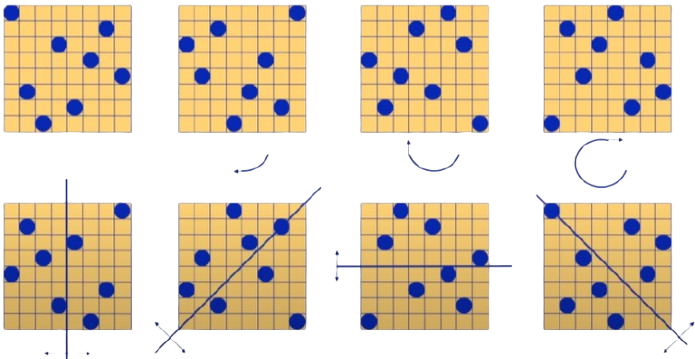
\includegraphics[height=50mm]{images/nqueens3.png}% 
  \end{center}    
\end{frame}

\begin{frame}
  \begin{example}[Continued]
    The symmetries of 8-queens are the following:

    \scriptsize
    \[
    \begin{array}{@{}ll@{}}
    \makebox[2em][l]{\text{id:}} 
      \left(
      \begin{array}{ccccccccc}
      q_1 & q_2 & q_3 & q_4 & q_5 & q_6 & q_7 & q_8 & q_9 \\
      q_1 & q_2 & q_3 & q_4 & q_5 & q_6 & q_7 & q_8 & q_9
      \end{array}
      \right) &
    \makebox[2em][l]{\text{r90:}} 
      \left(
      \begin{array}{ccccccccc}
      q_1 & q_2 & q_3 & q_4 & q_5 & q_6 & q_7 & q_8 & q_9 \\
      q_7 & q_4 & q_1 & q_8 & q_5 & q_2 & q_9 & q_6 & q_3
      \end{array}
      \right) \\[3em]
      
    \makebox[2em][l]{\text{r180:}} 
      \left(
      \begin{array}{ccccccccc}
      q_1 & q_2 & q_3 & q_4 & q_5 & q_6 & q_7 & q_8 & q_9 \\
      q_9 & q_8 & q_7 & q_6 & q_5 & q_4 & q_3 & q_2 & q_1
      \end{array}
      \right) &
    \makebox[2em][l]{\text{r270:}} 
      \left(
      \begin{array}{ccccccccc}
      q_1 & q_2 & q_3 & q_4 & q_5 & q_6 & q_7 & q_8 & q_9 \\
      q_3 & q_6 & q_9 & q_2 & q_5 & q_8 & q_1 & q_4 & q_7
      \end{array}
      \right) \\[3em]
      
    \makebox[2em][l]{\text{x:}} 
      \left(
      \begin{array}{ccccccccc}
      q_1 & q_2 & q_3 & q_4 & q_5 & q_6 & q_7 & q_8 & q_9 \\
      q_3 & q_2 & q_1 & q_6 & q_5 & q_4 & q_9 & q_8 & q_7
      \end{array}
      \right) &
    \makebox[2em][l]{\text{y:}} 
      \left(
      \begin{array}{ccccccccc}
      q_1 & q_2 & q_3 & q_4 & q_5 & q_6 & q_7 & q_8 & q_9 \\
      q_7 & q_8 & q_9 & q_4 & q_5 & q_6 & q_1 & q_2 & q_3
      \end{array}
      \right) \\[3em]
      
    \makebox[2em][l]{\text{d1:}} 
      \left(
      \begin{array}{ccccccccc}
      q_1 & q_2 & q_3 & q_4 & q_5 & q_6 & q_7 & q_8 & q_9 \\
      q_1 & q_4 & q_7 & q_2 & q_5 & q_8 & q_3 & q_6 & q_9
      \end{array}
      \right) &
    \makebox[2em][l]{\text{d2:}} 
      \left(
      \begin{array}{ccccccccc}
      q_1 & q_2 & q_3 & q_4 & q_5 & q_6 & q_7 & q_8 & q_9 \\
      q_9 & q_6 & q_3 & q_8 & q_5 & q_2 & q_7 & q_4 & q_1
      \end{array}
      \right)
    \end{array}
    \]
  \end{example}
\end{frame}

\begin{frame}{Value and variable symmetry}
  \begin{definition}
    A \defined{value symmetry} is a permutation of the values in a CSP that \defined{preserves all constraints and solutions}. For a given value symmetry $\sigma$, $[x_i = v \text{, } \forall \text{ } 1 \leq i < n]$ is symmetrical to $[x_i = \sigma(v) \text{, } \forall \text{ } 1 \leq i < n]$. If two values can be swapped without altering the set of solutions or violating any constraints, the CSP exhibits value symmetry.
  \end{definition}
  \vfill

  \begin{definition}
    A \defined{variable symmetry} $\sigma$ is a permutation of the decision variables in a CSP that \defined{preserves all constraints and solutions}. For a given variable symmetry $\sigma$, $[x_i = v \text{, } \forall \text{ } 1 \leq i < n]$ is symmetrical to $[\sigma(x_i) = v \text{, } \forall \text{ } 1 \leq i < n]$.
    If two variables can be swapped without changing the set of solutions or violating any constraints, the CSP exhibits variable symmetry.
  \end{definition}

  As with the variable symmetries in the example with $n$-queens 
\end{frame}

\begin{frame}
  \begin{example}[Value symmetry: map coloring]
    Use $k$ colours to paint the countries of a map such that no
    neighbour countries have the same colour. \\[+5pt] The
    model where the countries (as decision variables) take colours (as
    values) has $k!$ \defined{value symmetries} because any
    permutation of the colours transforms a (non-)solution into
    another (non-)solution: the values are not distinguished.
  \end{example}
  \vfill

  Symmetric colouring of graphs:
  \vfill

  \begin{columns}
    \begin{column}{0.33\textwidth}
      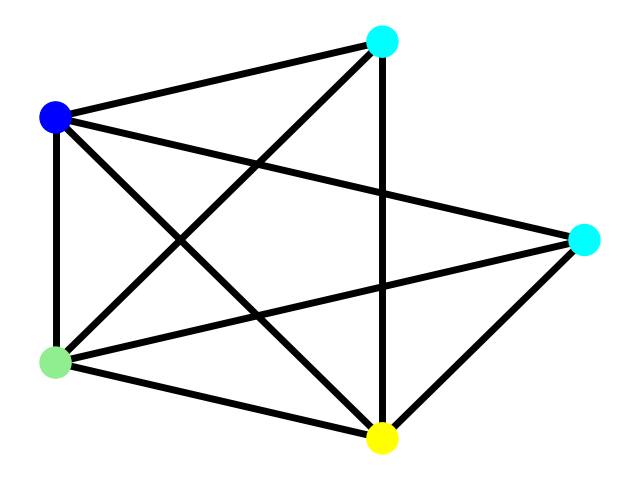
\includegraphics[height=35mm]{images/graph1.png}%
    \end{column}
    

    \begin{column}{0.33\textwidth}
      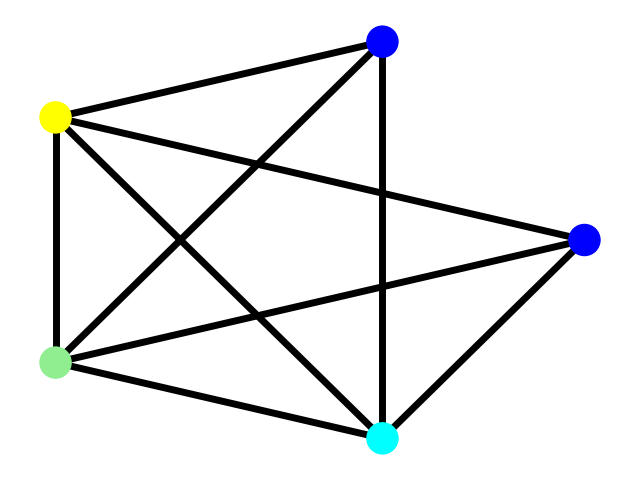
\includegraphics[height=35mm]{images/graph2.png}%          
    \end{column}
    

    \begin{column}{0.33\textwidth}
      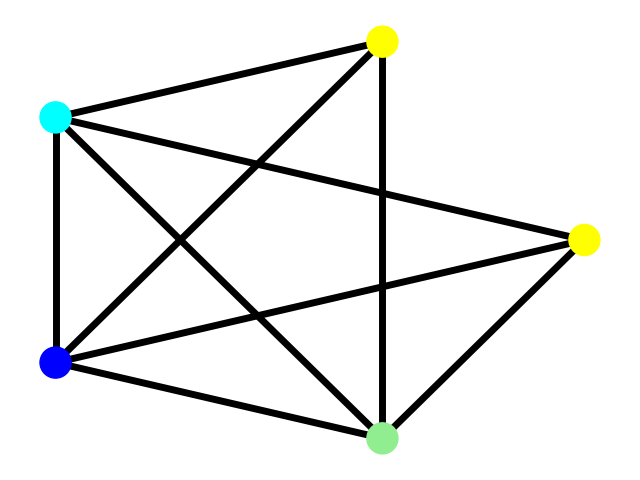
\includegraphics[height=35mm]{images/graph3.png}%          
    \end{column}
  \end{columns}
\end{frame}

\begin{frame}
  \begin{example}[Variable symmetry: subset problem]
    Problem definition: Find an $n$-element subset of a given set $S$, subject to some
    constraints. 
    \\[+8pt]  
    The model encoding the subset as an
    array of $n$ integer decision variables of domain~$S$, constrained to take
    distinct values, has \\  $n!$~\defined{variable symmetries} as the
    order of the elements does not matter in a set, but does matter in
    an array. 
    \\[+8pt]     
    Assume $n=3$. there are 6 variable symmetries: \\
    Solution \cpminline{[1,2,3]} (i.e., \cpminline{x1 = 1, x2 = 2, x3 = 3}) \\
    is symmetric to solutions \\\cpminline{[1,3,2], [2,1,3], [2,3,1], [3,2,1], [3,1,2]}
  \end{example}
\end{frame}

\begin{frame}{Variable symmetriy special case: Index symmetry}
  Index symmetry is a special case of variable symmetry, occurring on slices of a tensor of decision variables.

  \begin{definition}
    \defined{Index symmetry}: occurs in problems involving arrays or matrices of decision variables; permutations of \textbf{slices} of an
      array of decision variables preserve all constraints and solutions. 
  \end{definition}
  \vfill
    
  Common cases: \defined{row symmetry}, \defined{column symmetry} \dots
  \vfill

  \structured{Careful: Index symmetries multiply up!} \\ If there is
  full row and column symmetry in an $m \times n$ array \\ (that is,
  if there are $m!$ row symmetries and $n!$ column symmetries), \\
  then there are $m! \cdot n!$~compositions of
  symmetries. 
\end{frame}

\begin{frame}{Variable symmetry special case: Index symmetry}
  \begin{example}[Latin Squares]
    Construct an $n \times n$ Latin square where each row and column contains each number from 1 to $n$ exactly once. \\[+5pt]
    The problem has $n!^2$ \defined{index symmetries} because any permutation of the rows or columns ($n!$ permuations each) transforms a (non-)solution into another (non-)solution: the indices are not distinguished.
  \end{example}
  \vfill

  \begin{columns}
    \begin{column}{0.3\textwidth}
      \centering A solution 
      \[
      \begin{array}{|c|c|c|c|}
      \hline
      1 & 2 & 3 & 4 \\
      \hline
      2 & 3 & 4 & 1 \\
      \hline
      3 & 4 & 1 & 2 \\
      \hline
      4 & 1 & 2 & 3 \\
      \hline
      \end{array}
      \]        
    \end{column}
    

    \begin{column}{0.3\textwidth}
      \quad Swap rows 1 and 2
      \[
      \begin{array}{|c|c|c|c|}
        \hline
        2 & 3 & 4 & 1 \\
        \hline
        1 & 2 & 3 & 4 \\
        \hline
        3 & 4 & 1 & 2 \\
        \hline
        4 & 1 & 2 & 3 \\
        \hline
      \end{array}
      \]        
    \end{column}
    

    \begin{column}{0.3\textwidth}
      Swap columns 1 and 2
      \[
      \begin{array}{|c|c|c|c|}
      \hline
      2 & 1 & 3 & 4 \\
      \hline
      3 & 2 & 4 & 1 \\
      \hline
      4 & 3 & 1 & 2 \\
      \hline
      1 & 4 & 2 & 3 \\
      \hline
      \end{array}
      \]        
    \end{column}    
  \end{columns}
\end{frame}

\begin{frame}{Symmetries}
  What is the origin of the symmetries?
  \vfill
  
  \structured{Symmetries can be present due to different reasons} 
  \vfill

  \begin{itemize}
    \item Problem symmetries \vfill
    \item Instance symmetries \vfill
    \item Model symmetries
  \end{itemize}
\end{frame}

\begin{frame}{Problem symmetries}
  \begin{definition}
    A \defined{problem symmetry} is a symmetry of a CSP that is inherent to the problem itself and is detectable in \textit{every model} of the problem. 
  \end{definition}
  \vfill

  The symmetries in map colouring and $n$-queens we discussed are \defined{problem symmetries}:
  \vfill

  \begin{itemize}
    \item The values in graph colouring do not represent entities with different attributes; the actual colour does not matter.
      \vfill
    \item The variables in $n$-queens represent the queens with the same characteristics.
      \vfill
    \item Both the tasks and the machines in the scheduling problem are indistinguishable, thus symmetric.
  \end{itemize}
\end{frame}

\begin{frame}{Instance symmetries}
  \begin{definition}
    An \defined{instance symmetry} is a symmetry detectable in a specific instance of a CSP. These symmetries depend on the particular values or structure of the instance rather than the general problem or its model.
  \end{definition}
  \vfill

  \begin{example}[Graph colouring]
    \small
    \raisebox{-\height}[0pt][0pt]{%
      \begin{columns}
        \begin{column}{0.65\textwidth}
            
        \end{column}
        \begin{column}{0.3\textwidth}
          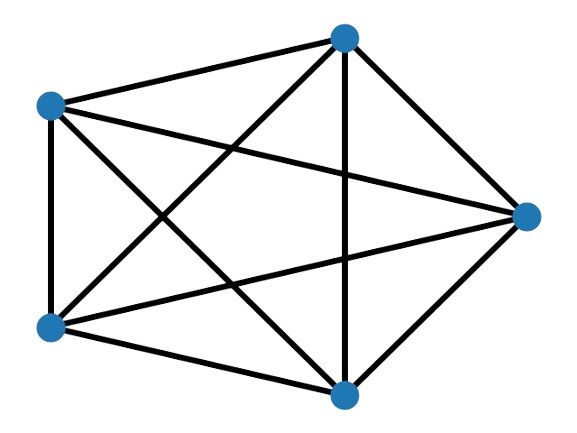
\includegraphics[height=22mm]{images/graph_clique.png}%
        \end{column}
      \end{columns}
    }

    \textit{\textbf{Problem}}: Use $k$ colours to paint the nodes of a graph \\such that no neighbour nodes have the same colour. \\[+5pt]
    \textit{\textbf{Instance}}: Use $5$ colours to paint 5 nodes that are all \\neighbours with each other (i.e., they form a clique). \\[+5pt]
    
    \textit{\textbf{Symmetry}}: Besides the \blue{value symmetry} that is inherent to the graph colouring problem, we also have \blue{variable symmetry} in this instance due to its structure: All variables have the same properties and thus are symmetric! Permuting the assignment of any 2 variables converts a (non-)solution to a (non-)solution.    
  \end{example}
\end{frame}

\begin{frame}{Model symmetries}
  \begin{definition}
    A \defined{model symmetry} is a symmetry that arises from a specific representation of a CSP and is not detectable in every model of the problem. 
  \end{definition}    
  \vfill

  The symmetries in the subset model are \emph{not} problem symmetries \\
  but \defined{model symmetries}: they are \emph{not} present for every modeling choice.
  

  \begin{example}
    \textbf{Subset problem}: Find an $n$-element subset of a given set $S$, subject to some constraints. \\[+5pt] The model using boolean variables $B$, with $B_i$ representing if element $i$ is part of the subset, does not have the variable symmetries of the integer model! 
  \end{example}
  \vfill
          
  Model symmetries are \textbf{\textit{introduced}} during modeling and can be avoided by using a different model (to be discussed further).
\end{frame}


\section{Symmetry Breaking}

\begin{frame}{Symmetries affect solving time}
  \structured{Observation:} 
  \vfill

  \begin{itemize}
    \item 
      A solver may waste a lot of effort on backtracking over
      gazillions of (partial) \alert{non-solutions} that are symmetric to already visited ones
      \vfill
    \item 
      a found \alert{solution} can
      be transformed without search into a symmetric solution in
      polynomial time (i.e., much faster than \red{searching} for them).
  \end{itemize}
  \vfill

  \begin{block}{}
    \defined{Symmetry handling} has two aspects: \vfill
    \begin{itemize}
      \item \defined{Symmetry Detecting:} Detect (some) symmetries of the problem or instance \\
        or symmetries introduced when modelling.
      \vfill
      \item \defined{Symmetry Breaking:} Break (or better exploit) the
        detected symmetries so that less effort is spent on the
        solving: multiple symmetric representations of a (non-)solution are
        avoided.
    \end{itemize}
  \end{block}
  \vfill

  \alert{Automated symmetry detection is beyond the scope of this course.}
\end{frame}

\begin{frame}{Symmetry Breaking}
  \begin{definition}
    A \defined{symmetry class} is an equivalence class of solutions
    under all the considered symmetries, including their compositions.
  \end{definition}

  Solutions of the same symmetry class in graph colouring:
  \begin{columns}
    \begin{column}{0.25\textwidth}
      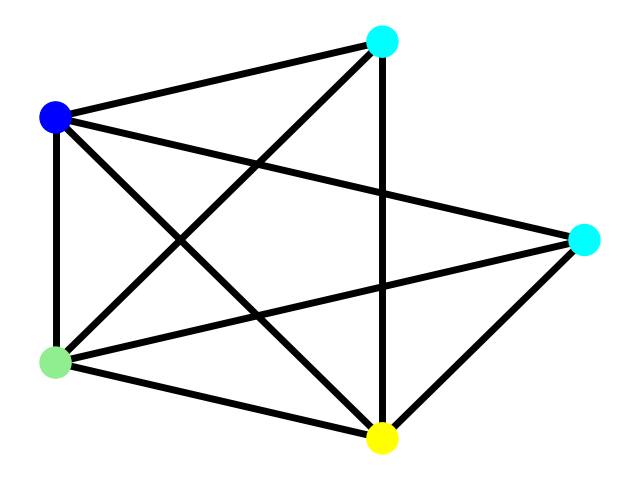
\includegraphics[height=25mm]{images/graph1.png}%
    \end{column}
    \begin{column}{0.25\textwidth}
      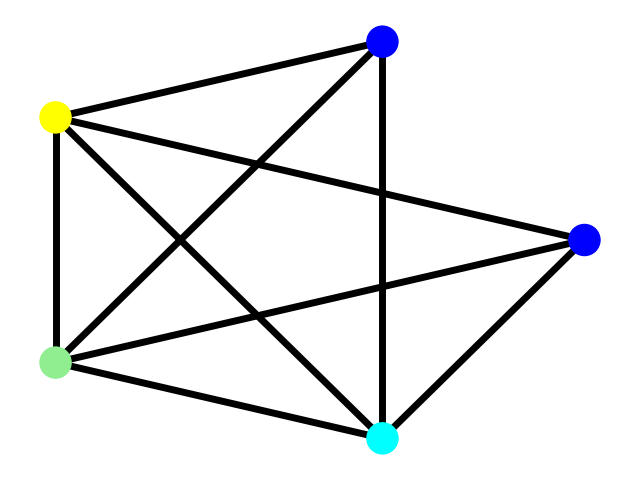
\includegraphics[height=25mm]{images/graph2.png}%          
    \end{column}
    \begin{column}{0.25\textwidth}
      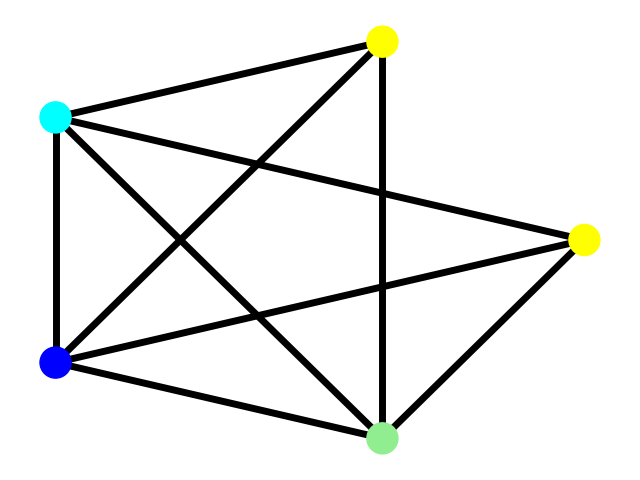
\includegraphics[height=25mm]{images/graph3.png}
    \end{column}
    \begin{column}{0.15\textwidth}
      \dots
    \end{column}
  \end{columns}
  \vfill
  
  \structured{Aim of Symmetry Breaking:} While solving, keep ideally \alert{one} member (i.e., solution) per
  symmetry class; this can significantly reduce the \search{search space}!
  \vfill

  \structured{Careful: Size does not matter!} \\
  The number of symmetries is \alert{no} indicator of the difficulty of breaking them!
\end{frame}

\begin{frame}{Symmetry Breaking}
  Breaking symmetries can be done in different ways.
  \vfill

  Types of symmetry breaking:
  \begin{itemize}
    \item \defined{Symmetry breaking by reformulation}: \\ the
      elimination of the symmetries detectable in the model.
    \item \defined{Static symmetry breaking}: \\ the elimination of
      symmetric solutions by adding \inference{constraints} upfront.
    \item \defined{Dynamic symmetry breaking}: \\ the elimination of
      symmetric solutions dynamically during \search{search}. (Out of scope)
  \end{itemize}
\end{frame}

\begin{frame}{Symmetry Breaking}
  Regardless of the type of symmetry breaking used, \\ our method needs to be \defined{sound} and \defined{efficient}:
  \vfill

  \begin{itemize}
    \item \defined{Soundness}: Symmetry breaking must keep \textbf{\textit{at least one}} solution from each symmetry class.
      \vfill 

    \item \defined{Efficiency}: Symmetry breaking should keep as few solutions as possible from each symmetry class. \\
    \alert{Ideally only 1!}
  \end{itemize}
\end{frame}


\subsection{Symmetry Breaking by Reformulation}

\begin{frame}{Breaking model symmetries by reformulation}
  \begin{definition}[recap]
    A \defined{model symmetry} is a symmetry that arises from a specific representation of a CSP and is not detectable in every model of the problem. 
  \end{definition}
  \vfill  

  We can break such symmetries by reformulating the model!
  \vfill

  \begin{example}
  	\small
    \textbf{Subset problem}: Find an $n$-element subset of a given set $S$, subject to some
    constraints. 
    \\[+5pt]  
    The model encoding the subset as an
    array of $n$ decision variables of domain~$S$, constrained to take
    distinct values, has \\  $n!$~\defined{variable symmetries}: the
    order of the elements does not matter \dots
    \\[+5pt]  
    We can reformulate the model to use boolean variables $B$, with $B_i$ representing if element $i$ is part of the subset, does not have the variable symmetries of the integer model! 
  \end{example}
\end{frame}


\subsection{Symmetry Breaking by Constraints}

\begin{frame}{Symmetry Breaking by Constraints}
  Often, not all symmetry can be eliminated by remodelling.
  \vfill

  Remaining symmetry should be reduced or eliminated.
  \vfill

  \begin{itemize}
    \item Static symmetry breaking: Using symmetry-breaking constraints.
      \begin{itemize}
        \item Different than implied constraints, as they \alert{change the set of solutions}
        \item Breaking symmetries with constraints can allow for further implied constraints
      \end{itemize}
      \vfill
    \item Dynamic symmetry-breaking methods during search. (out of scope)
  \end{itemize}
\end{frame}

\begin{frame}{Adding symmetry-breaking constraints}
  The added constraints must not exclude any non-symmetric solutions. The goal is to reduce redundancy without affecting the completeness of the search.\\[+5pt]
  \begin{itemize}
    \item \defined{Soundness}: Symmetry breaking must keep \textbf{\textit{at least one}} solution from each symmetry class.
  \end{itemize}
  \vfill 

  The added constraints should reduce the number of symmetric assignments that will be explored.\\[+5pt]
  \begin{itemize}
    \item \defined{Efficiency}: Symmetry breaking should keep as few solutions as possible from each symmetry class. \\ \alert{Ideally only 1!}
  \end{itemize}
\end{frame}

\begin{frame}{Lexicographic symmetry-breaking constraints}
  A common way to break symmetries is to impose a lexicographic ordering.
  \vfill

  Breaking \structured{variable symmetries}: lexicographic ordering on the variables.
  \vfill

  \begin{itemize}
    \item  enforcing an order in the variables, they are no longer indistinguishable and thus not symmetric. 
    \item May also have an effect on value symmetries: (Integer) values have an order that is now important!
  \end{itemize}
  \vfill

  Breaking \structured{index symmetries}: lexicographic ordering on the tensor slices.
  \begin{itemize}
    \item Row symmetries: lexicographic ordering of rows.
    \item Column symmetries: lexicographic ordering of columns.
    \item \dots
  \end{itemize}
  \vfill

  Powerful lexicographic symmetry-breaking \blue{global constraints} exist in CP.
\end{frame}

\begin{frame}{Lexicographic ordering on variables}
  \begin{example}[Golomb Rulers]
    \raisebox{-\height}[0pt][0pt]{%
      \begin{columns}
        \begin{column}{0.65\textwidth}
            
        \end{column}
        \begin{column}{0.2\textwidth}
          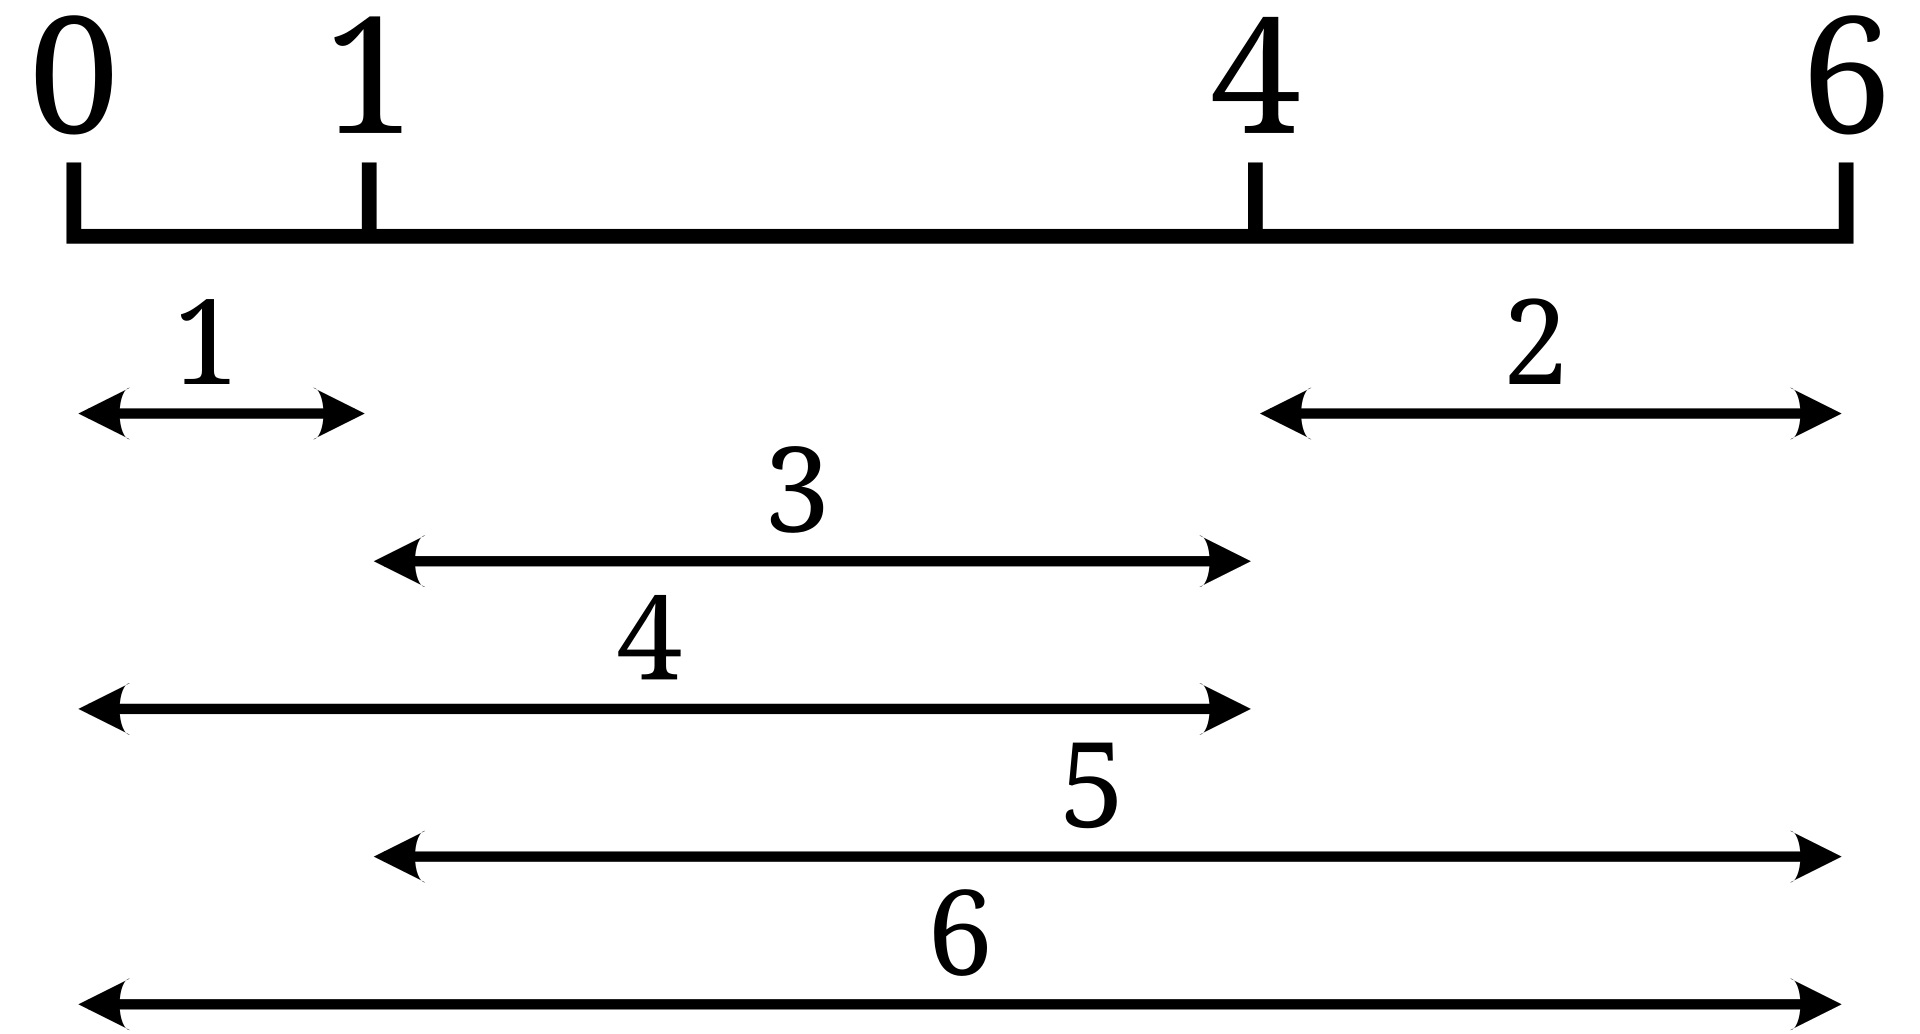
\includegraphics[height=18mm]{images/Golomb_Ruler-4.png}%
        \end{column}
      \end{columns}
    }

    A Golomb ruler has \(m\) marks, where all the \(\frac{m(m-1)}{2}\) distances \\ between marks (\(x_j - x_i \text{ } \forall \text{ } 0 < i,j <= m\)) are different
    \vfill

    \begin{itemize}
      \item Variables: one for each mark \(x_1, x_2, \ldots, x_m\)
      \item Constraints: \(x_j - x_i \neq x_l - x_k\) for all distinct pairs
        \vfill
      \item \structured{Variable Symmetry}: Variables are symmetrical. Solution $[0,1,4,6]$ is equivalent to $[0,4,1,6]$, and $[1,0,4,6]$, and \dots
        \vfill
      \item \defined{Symmetry breaking}: Enforce lexicographic ordering with 
        \(x_1 < x_2 < \ldots < x_m\)
         \\ [+5pt]
        Or directly use the \cons{IncreasingStrict}{X} global constraint for symmetry-breaking!
    \end{itemize}
  \end{example}
\end{frame}

\begin{frame}{Global constraints for lexicographic ordering of variables}
  \begin{definition}
    The \cons{Increasing}{X} global constraint holds if and only if the variables in $X$ are in an increasing order: 
    $$X_i \leq X_j \text{ } \forall \text{ } 0 \leq i < j < |X|$$
  \end{definition}
  \vfill

  \begin{definition}
    The \cons{Decreasing}{X} global constraint holds if and only if the variables in $X$ are in a decreasing order:
    $$X_i \geq X_j \text{ } \forall \text{ } 0 \leq i < j < |X|$$
  \end{definition}
  \vfill

  Similarly, the constraints \cons{IncreasingStrict}{X} and \cons{DecreasingStrict}{X} enforce a strict lexicographic order.
\end{frame}

\begin{frame}{Breaking index symmetries}
  \begin{example}[Latin Squares]
    \footnotesize
    A latin square of size $n \times n$ requires that each row and column contain each number from 1 to $n$ exactly once. 
    \vfill

    \begin{columns}
      \begin{column}{0.3\textwidth}
        \centering A solution 
        \[
        \begin{array}{|c|c|c|c|}
          \hline
          1 & 2 & 3 & 4 \\
          \hline
          2 & 3 & 4 & 1 \\
          \hline
          3 & 4 & 1 & 2 \\
          \hline
          4 & 1 & 2 & 3 \\
          \hline
        \end{array}
        \]        
      \end{column}
      \begin{column}{0.3\textwidth}
        \centering Swap rows 1 and 2
        \[
        \begin{array}{|c|c|c|c|}
          \hline
          2 & 3 & 4 & 1 \\
          \hline
          1 & 2 & 3 & 4 \\
          \hline
          3 & 4 & 1 & 2 \\
          \hline
          4 & 1 & 2 & 3 \\
          \hline
        \end{array}
        \]        
      \end{column}
      \begin{column}{0.3\textwidth}
        \centering Swap columns 1 and 2
        \[
        \begin{array}{|c|c|c|c|}
          \hline
          2 & 1 & 3 & 4 \\
          \hline
          3 & 2 & 4 & 1 \\
          \hline
          4 & 3 & 1 & 2 \\
          \hline
          1 & 4 & 2 & 3 \\
          \hline
        \end{array}
        \]        
      \end{column}    
    \end{columns}
  \end{example}
  \vfill

  \structured{Lexicographic ordering of lists}: $X \LeqLex Y$, with $X,Y$ being lists. 
  \vfill

  Compare the lists element by element from left to right; the first differing element determines the order.
  \vfill

  Slices of tensors are lists, so we can use the $\LeqLex$ operator.
\end{frame}

\begin{frame}{Breaking index symmetries}
  \begin{example}
    $[1,2,34,5,678] \LeqLex [1,2,36,45,78]$) \\
    because $34 < 36$, even though~
    $678 \not\leq 78$: this $\LeqLex$ order on
    1d integer arrays does not require \textit{all} elements to be less than or equal to the corresponding element in the other array; It only considers the first differing pair.
  \end{example}\vfill
  
  \begin{definition}[\cons{LexLess}{} and \cons{LexLessEq}{} global constraints]
    The \cons{LexLess}{X,Y} (resp. \cons{LexLessEq}{X,Y}) constraint, where $X$
    and $Y$ are same-length lists (or 1D arrays) of decision variables, with size $n$,
    holds if and only if $X$ is lexicographically less (resp. less or equal) to $Y$:
    \begin{itemize}
      \item either~ $n = 0$,
      \item or~ $X_1 < Y_1$,
      \item or~ $X_1 = Y_1$ \& \cons{LexLess}{$[X_i \forall i \in [2..n]], [Y_j \forall j \in  [2..n]]$}.
      \begin{itemize}
        \item resp. $X_1 = Y_1$ \& \cons{LexLessEq}{$[X_i \forall i \in [2..n]], [Y_j \forall j \in  [2..n]]$}.
      \end{itemize}
    \end{itemize}
  \end{definition}
\end{frame}

\begin{frame}{Breaking index symmetries}
  Lexicographic ordering constraints along \alert{one} dimension of an array \\
  break the index symmetry of that dimension. \vfill
  
  \begin{example}[Latin Squares]
    \small
    A latin square of size $n \times n$ requires that each row and column contain each number from 1 to $n$ exactly once. 
    \vfill

    \begin{columns}
      \begin{column}{0.3\textwidth}
        \centering A solution 
        \[
        \begin{array}{|c|c|c|c|}
          \hline
          1 & 2 & 3 & 4 \\
          \hline
          2 & 3 & 4 & 1 \\
          \hline
          3 & 4 & 1 & 2 \\
          \hline
          4 & 1 & 2 & 3 \\
          \hline
        \end{array}
        \]        
      \end{column}

      \begin{column}{0.3\textwidth}
        \centering Swap rows 1 and 2
        \[
        \begin{array}{|c|c|c|c|}
          \hline
          2 & 3 & 4 & 1 \\
          \hline
          1 & 2 & 3 & 4 \\
          \hline
          3 & 4 & 1 & 2 \\
          \hline
          4 & 1 & 2 & 3 \\
          \hline
        \end{array}
        \]        
      \end{column}

      \begin{column}{0.3\textwidth}
        \centering Swap columns 1 and 2
        \[
        \begin{array}{|c|c|c|c|}
          \hline
          2 & 1 & 3 & 4 \\
          \hline
          3 & 2 & 4 & 1 \\
          \hline
          4 & 3 & 1 & 2 \\
          \hline
          1 & 4 & 2 & 3 \\
          \hline
        \end{array}
        \]        
      \end{column}    
    \end{columns}
    \vfill

    \alert{Latin squares problem has both row and column symmetries!} 
    \\[+5pt]
    Assume variables $X_{ij}$ with $i,j \in [1..n]$.
    Breaking the row symmetries:

    $$\cons{LexLess}{[X_{ij} \text{ } \forall \text{ } j \in [1..n]] , [X_{i+1,j} \text{ } \forall \text{ } j \in [1..n]]} \text{ } \forall \text{ } i \in [1..n-1]$$
  \end{example}
\end{frame}

\begin{frame}\label{lex2:counterex}
  Lexicographic ordering constraints along \alert{every} dimension
  with index symmetry of an array have two properties:
  \begin{itemize}
    \item[$+$] No symmetry class is lost. At least one solution remains from each class.
    \item[$-$] In general, \alert{not} all symmetry classes are left with $1$ solution, \\ except if the values of the array are distinct, etc.
  \end{itemize} \vfill
  \begin{block}{Counterexample}
    Assume full row symmetry and full column symmetry: \\ the arrays
    \begin{tabular}{|c|c|c|}
      \hline
      0 & 0 & 1 \\
      \hline
      1 & 1 & 0 \\
      \hline
    \end{tabular}
    and
    \begin{tabular}{|c|c|c|}
      \hline
      0 & 1 & 1 \\
      \hline
      1 & 0 & 0 \\
      \hline
    \end{tabular}
    have lexicographically ordered rows \alert{and} columns, but are
    symmetric: each can be transformed into the other by swapping
    their two rows as well as swapping their first and last columns.
  \end{block}
  \vfill
  
  General scheme for breaking all variable symmetries: The \defined{Lex-Leader} scheme (see next slide) generates lexicographic ordering constraints that are not necessarily along the dimensions
  of an array of decision variables. \\ 
  \alert{It guarantees that all the compositions of all variable symmetries are broken}.
\end{frame}

\begin{frame}{The Lex-Leader Scheme}\label{lex-leader}
  \blue{Main idea} of the \defined{Lex-Leader} scheme: 
  \begin{itemize}
    \item For each equivalence class of solutions
      under our symmetry group, predefine \textit{one} to be the canonical solution.
    \item Achieves this by adding constraints that are satisfied by canonical solutions and not by symmetric ones.
  \end{itemize}
  \vfill

  For each permutation in a given symmetry group $G$, \defined{Lex-Leader} produces one lexicographic constraint. 
  \vfill

  The set of constraints defined by the \defined{Lex-Leader} method, using the lexicographic relation $\LeqLex$ in a symmetry group $G$ with a chosen variable ordering $V$, is
  $$\forall \sigma \in G, V \LeqLex \sigma(V)$$

  where $V$ is the vector of the variables of the CSP (in a defined order), and $\LeqLex$ is the lexicographic ordering
  relation
\end{frame}

\begin{frame}[fragile]{The Lex-Leader Scheme}
  For \alert{any} group $G$ of \alert{variable} symmetries on the
  indices of the decision variables $x_1,\dots,x_n$ of
  domain $D$, which are not necessarily arranged into a 1d array:
  \vfill

  \begin{enumerate}
    \item Choose an ordering of the decision variables, say
      $x_1,\dots,x_n$.  \vfill
    \item Choose a lexicographic-ordering relation,  say \mzninline{lex_lesseq}. \vfill
    \item For every symmetry $\sigma \in G$, add a constraint enforcing the lexicographic relation
      $$LexLessEq([x_1,\dots,x_n],[\sigma(x_1),\dots,\sigma(x_n)])$$
      to the problem model. \vfill
    \item Simplify the resulting constraints, locally and globally.
  \end{enumerate}\vfill

  This yields \alert{exactly} one solution per symmetry class.
\end{frame}

\begin{frame}[fragile]
  \begin{example}[$2 \times 3$ array with full row and column symmetry]
    \small
    Consider the array
    \begin{tabular}{|c|c|c|}
      \hline
      \texttt{x1} & \texttt{x2} & \texttt{x3} \\
      \hline
      \texttt{x4} & \texttt{x5} & \texttt{x6} \\
      \hline
    \end{tabular}
    with full row and column symmetry: Need
    $2!$ (from column symmetry) $ \cdot 3!$ (from row symmetry) $ - 1 = 11$ constraints for the ordering
    $x_1,x_2,x_3,x_4,x_5,x_6$:
\\[+10pt]
1. \cons{LexLessEq}{$[x_1,x_2,x_3,x_4,x_5,x_6],[x_2,x_1,x_3,x_5,x_4,x_6]$} (for cols 1-2)  

2. \cons{LexLessEq}{$[x_1,x_2,x_3,x_4,x_5,x_6],[x_1,x_3,x_2,x_4,x_6,x_5]$} (for cols 2-3)  

3. \cons{LexLessEq}{$[x_1,x_2,x_3,x_4,x_5,x_6],[x_4,x_5,x_6,x_1,x_2,x_3]$} (for rows)  

4. \cons{LexLessEq}{$[x_1,x_2,x_3,x_4,x_5,x_6],[x_6,x_4,x_5,x_3,x_1,x_2]$} (for rows + cols 2-3, 1-2)  

5. \cons{LexLessEq}{$[x_1,x_2,x_3,x_4,x_5,x_6],[x_5,x_6,x_4,x_2,x_3,x_1]$} (for rows + cols 1-2, 2-3)  

6. \cons{LexLessEq}{$[x_1,x_2,x_3,x_4,x_5,x_6],[x_4,x_6,x_5,x_1,x_3,x_2]$} (for rows + cols 2-3)  

7. \cons{LexLessEq}{$[x_1,x_2,x_3,x_4,x_5,x_6],[x_5,x_4,x_6,x_2,x_1,x_3]$} (for rows + cols 1-2)  

8. \cons{LexLessEq}{$[x_1,x_2,x_3,x_4,x_5,x_6],[x_6,x_5,x_4,x_3,x_2,x_1]$} (for rows + cols 1-3)  

9. \cons{LexLessEq}{$[x_1,x_2,x_3,x_4,x_5,x_6],[x_3,x_2,x_1,x_6,x_5,x_4]$} (for cols 1-3)  

10. \cons{LexLessEq}{$[x_1,x_2,x_3,x_4,x_5,x_6],[x_2,x_3,x_1,x_5,x_6,x_4]$} (for cols 1-2, 2-3)  

11. \cons{LexLessEq}{$[x_1,x_2,x_3,x_4,x_5,x_6],[x_3,x_1,x_2,x_6,x_4,x_5]$} (for cols 2-3, 1-2)  

  \end{example}
\end{frame}

\begin{frame}{Symmetry Breaking}
  The Lex-Leader Scheme is general, but takes exponential
  space if there are exponentially many symmetries!
  \vfill

  Problem-specific symmetry-breaking constraints may be more beneficial.
  \vfill

  Note: Breaking \alert{all} the symmetries may increase the solving time:
  \begin{itemize}
    \item More propagation time than reduction in search time
    \item Break only \alert{some} symmetries, but which ones?
  \end{itemize}
  \vfill

  Often problem and model specific.
\end{frame}


\section{Dominance Breaking}

\begin{frame}{Dominance Breaking}
  \small
  \begin{itemize}
    \item Symmetry breaking can be beneficial also for optimization problems\\ (for any symmetric solutions $s_1, s_2$ we have $f(s_1) = f(s_2)$); 
    \vfill
    
    \item But we can \textit{generalize} the concept of symmetry breaking in optimization problems.
    \vfill
    
    \item In optimization problems, the \textit{minimization} of an objective function $f$ determines optimality; exploring \red{suboptimal} assignments should be avoided.
    \vfill
    
    \item Many constraint problems exhibit \defined{dominance relations} which can be exploited for dramatic \red{reductions in search space}.
  \end{itemize}
  \vfill 
  \begin{definition}
    Given a problem with an objective function $f$, \defined{a dominance relation} $\prec$ is a binary relation on the set of solutions $S$, such that if $s_1 \prec s_2$ for $s_1, s_2 \in S$, then one of the following is true:
    \begin{enumerate} 
      \item $s_1$ is a solution and $s_2$ is not.
      \item They are both solutions and $f(s_1) < f(s_2)$.
      \item They are both non-solutions and $f(s_1) < f(s_2)$.
    \end{enumerate}  
  \end{definition}
\end{frame}

\begin{frame}{Dominance Breaking}
  \blue{Main idea}: A (partial) assignment that satisfies the constraints can be forbidden if it is dominated.
  \begin{itemize}
    \item for any solution that this assignment would lead to, there must be another solution that is equally good or better
  \end{itemize}
  \vfill

  Identify dominance relations in the problem that can be used to cut the search space.
  \vfill

  Add \defined{dominance-breaking} constraints to reduce the search space and speed up the solving process.
\end{frame}

\begin{frame}
  \begin{example}[Dominance]
    Consider a simple problem with:
    \begin{itemize}
      \item Domain: \( x_i \in \{1, \ldots, 10\} \),
      \item Constraint: \cons{AllDifferent}{[\(x_1, \ldots, x_{10}\)]},
      \item Objective function: \( \sum_{i=1}^{10} i \cdot x_i \) to be minimized.
    \end{itemize} 
    \vspace{5pt}
    
    The partial assignment \( s_1 = [x_1 = 2, x_2 = 1] \) \textbf{dominates} the partial assignment \( s_2 = [x_1 = 1, x_2 = 2] \), because:     \\[+5pt]
    No matter how we label the remaining variables, 
    the corresponding complete assignments \( s_1', s_2' \) with same values for \( x_3, \ldots, x_{10} \),
    will always have $f(s_1'), < f(s_2')$.
    \\[+5pt]
    This is due to:
    \[
    1 \cdot 2 + 2 \cdot 1 < 1 \cdot 1 + 2 \cdot 2.
    \]
  \end{example}
\end{frame}

\begin{frame}
  \begin{example}[Dominance Breaking]
    Identify the \defined{dominance} relation in the previous example:
    \\[+5pt]
    We have the objective function $f = \sum_{i=1}^{10} i \cdot x_i$.
    \\[+5pt]
    To minimize the \blue{objective}, we want higher values for variables with smaller indices because so that they have less impact on the total sum.
    \\[+5pt] 
    The following \defined{dominance} exists for this objective, without contradicting the constraint
    $$x_i \geq x_j, \text{ } \forall i < j$$
    \\[+5pt]
    Due to the \cons{AllDifferent}{} constraint, we can simplify it to
    $$x_i > x_j, \text{ } \forall i < j$$
    \\[+5pt] 
    By enforcing such a \textbf{lexicographic order} in our variables, dominated assignments will not be explored during the search process
  \end{example}
\end{frame}


\section{Recap}

\begin{frame}{Recap}
  Often symmetries exist in the problem, \search{wasting search effort}
  \begin{itemize}
    \item Variable and value symmetries.
  \end{itemize}
  \vfill

  Different types based on where symmetries are introduced:
  \begin{itemize}
    \item \defined{problem symmetries} are
      detectable in \emph{every} instance and model of the problem.
    \item \defined{instance symmetries} are
      detectable in \emph{specific instances} of a problem. \\
    \item \defined{model symmetries} are \emph{not}
      detectable in every model, but only in specific viewpoints.
  \end{itemize}
  \vfill

  Symmetry breaking is a very efficient method to \green{speed up} the solving process
  \vfill

  Powerful lexicographic \inference{global constraints} exist to break symmetries
  \vfill

  The \blue{Lex-Leader} scheme offers a general method to break symmetries
\end{frame}

\begin{frame}{Recap}
  \begin{itemize}
    \item Keep in mind the objective: first solution, all solutions, or best solution? \\
      Symmetry breaking might pay off more in some cases \\
      (Unsat, all solutions, optimal solution) \vfill
    
    \item Problem constraints can sometimes be simplified in the
      presence of symmetry-breaking constraints. \\
      \structured{Example:} $z = \cons{abs}{x-y}$ can be simplified
      into $z = x-y$ if symmetry-breaking requires
      $x \geq y$; $z = x-y$ is much easier for solvers than $z = \cons{abs}{x-y}$
      \vfill

    \item \blue{Dominance breaking} offers additional improvements for optimization problems!
  \end{itemize}
\end{frame}

\end{document}
